%--------------------------------------------------------------------
%
%Mustervorlage fuer eine Aufgabe
%
%--------------------------------------------------------------------
%
%Ueberschreiben der automatisch erzeugten Aufgabennummer
%Die folgende Aufgabennummer ergibt sich aus dem Stand des
%Z�hlers + 1
%\setcounter{chapter}{0}
%
\chapter{Methodology and Implementation}\label{chap:implementation}
%
%
%

This thesis consists of several components that run in unison to each other. Each component can be thought of as a building block to form a wall. To successfully build the wall each block must be carefully placed so that it effectively supports the next. In this chapter, the implementation and methodology of  each component will be explained.  

\section{Software architecture}
For a better understanding of the developed ROS software,  it's important to describe its architectural design and explain the connection between its different components. This section describes the overall ROS software architecture and the architecture of the implemented software.
 
In general, the architecture of any software which is based on ROS can be divided into two main layers. The first layer is the ROS computation graph. This computation graph contains nodes, topics, messages, and other components. The second layer is the ROS filesystem which contains all files and packages of the software.\citep{joseph_understanding_2015} A general example of the architecture design of a  software-based on ROS is shown in \ref{fig1}.  The components of each layer of the software are described and discussed in detail in the following sections. 

\begin{figure}[ht]
	\centering
	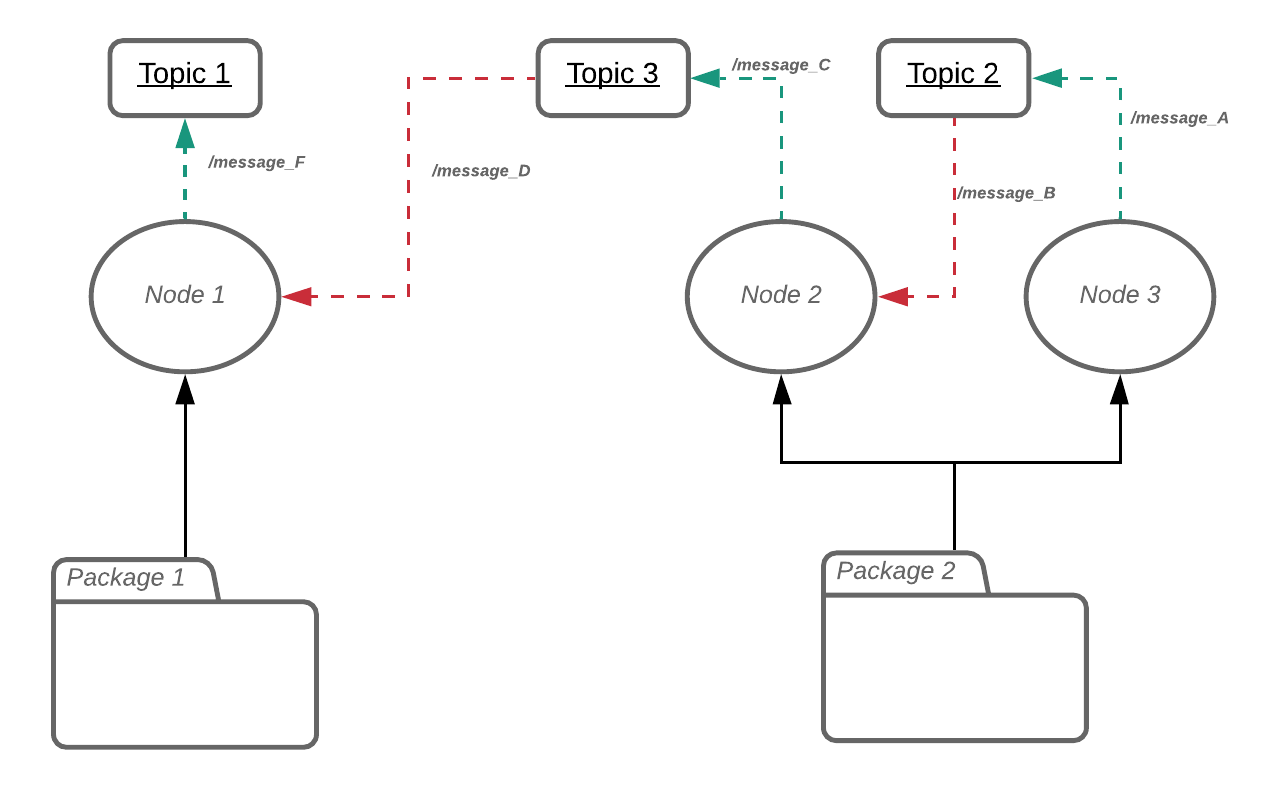
\includegraphics[width = 0.8\textwidth, frame]{./Bilder/UML_Architecture.png}			\caption{ROS architecture design}
	\label{fig1}
\end{figure}


\subsection{ROS filesystem:}


The top component of the filesystem is the catkin workspace which contains all used packages. Beneath the catkin workspace come the packages. The packages provide different tools and libraries, which could be used and configured to accomplish the desired functionalities. Each package contains messages, data types, services, and most importantly executable files and launch files \cite{joseph_understanding_2015}. The executable files, which are written either in C++ or in Python, are used to initialize ROS nodes. The launch files are used to configure and launch specific nodes. Since ROS is an open-source tool, all its packages can be found through the ROS Software Browser. During installation, there are some default packages that are recommended while downloading ROS. Other than this, all remaining packages must be downloaded or cloned individually from the Software Browser or alternatively be made from scratch. The following figure \ref{fig2} clearly demonstrates all the packages used in this project and the nodes that they include. 


\begin{figure}[ht]
	\centering
	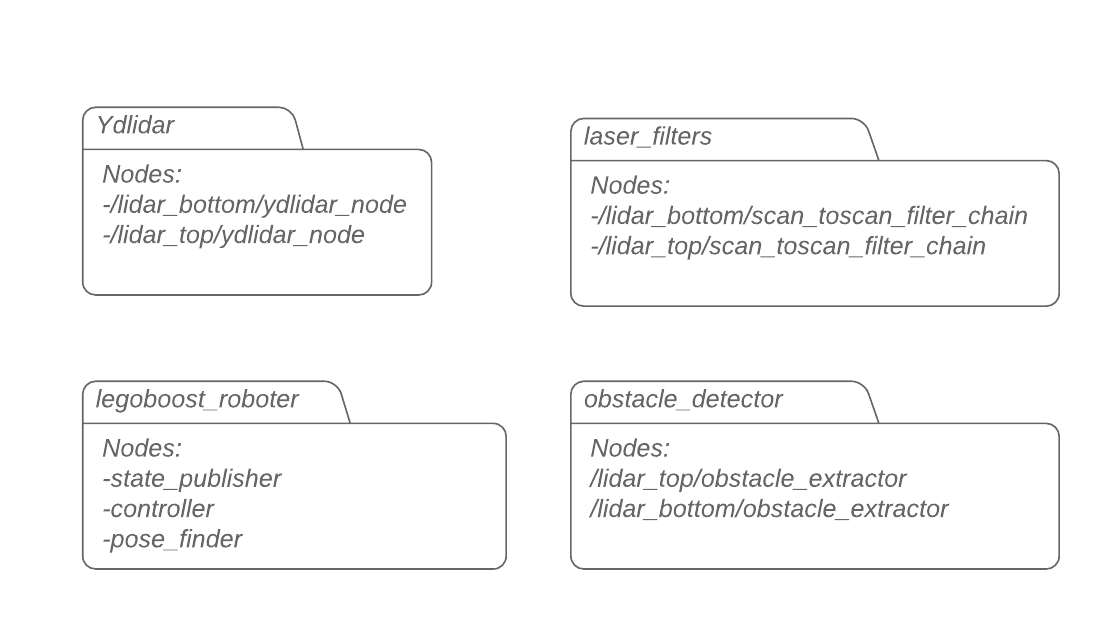
\includegraphics[width = 0.8\textwidth, frame]{./Bilder/UML_Packages.png}			\caption{ROS packages of the project}
	\label{fig2}
\end{figure}






Packages needed to be installed to support the default ROS packages are: 
\begin{enumerate}
\item \textbf{Ydlidar Package:} The first to be installed is the Ydlidar package, which supports the triangulation sensor package and is developed by Shenzhen EAI Technology Co. that produces. This has all the executable files that process the sensor data and publish it as a laserscan message to a topic. It also contains launch files for visualizing the sensor data in rviz. The nodes created in these packages are the /lidar-bottom/ydlidar-node contains all information about the bottom sensor while the /lidar-top/ydlidar-node contains all information about the top sensor. Further information about then nodes are discussed in the computation graph section \ref{subsec:computationGraph}.
\item  \textbf{The Laser-Filters Package:} this package is responsible for adjusting messages of type laserscan obtained from the triangulation sensor by using predefined filters so that it is suitable for later processing. Another option is to use pointCloud messages but this option is not required as the sensor publishes messages of type laserscan and not pointCloud. This package includes a node called scan-toscan-filter-chain, which is a pipeline of filters defined by the user \cite{foote_laser_filters_nodate}. It is useful for instances such as removing laser points off the wall in order to concentrate only on the robot laser scan data.
\item  \textbf{The Obstacle Detector Package:} This package is initially used for obstacle detection and tracking by using laserscan data from lidar sensors. However, in our case, this package is used to detect the robot. The node used in this package is called the obstacle-extractor node. This package also has a user-defined message type called "Obstacle" which includes the position of the obstacle in the XYZ plane. It also has nodes to visualize the obstacles in rviz. \cite{przybyla_tysikobstacle_detector_2020}
\item  \textbf{The Legoboost-Roboter Package:} Unlike the other packages, this one is made from scratch and contains all the information about the robot. This package consists of three main components; the controller, pose detector, and state publisher, each of which has a specific function. The state publisher consists of a node responsible for publishing the robots' frames and contains its URDF file. The pose detector is essentially a node that calculates the position and orientation of the robot using data collected from the obstacle collector. And lastly, the controller, which has a node that is responsible for the motion control of the robot.
\end{enumerate}





\subsection{ROS computation graph:}\label{subsec:computationGraph}



This section will go more in-depth on the computation graph layer for a better understanding of the software architecture. The computation graph is responsible for the connection between these components and the way the information is exchanged between these components. ROS node is one of the main components of the computation graph. It is responsible for computing a specific functionality or task.  ROS Nodes are connected together through topics or services. They could subscribe to topics to get the information from these topics and use this information to perform a specific task. They can also publish information to topics to post-process this information. Information that is exchanged between topics is called a message. Messages types can be either built-in, for example String or Bool, or can be defined by the user. \cite{joseph_learning_2018}. Figure \ref{fig3} shows the nodes used in this software and how they are interconnected. Any item within a square notions that this item is a topic, however an item within a circle relates to a node. This figure is generated by the rqt tool from ROS. This is a framework that is used for GUI purposes. 



\begin{figure}[ht]
	\centering
	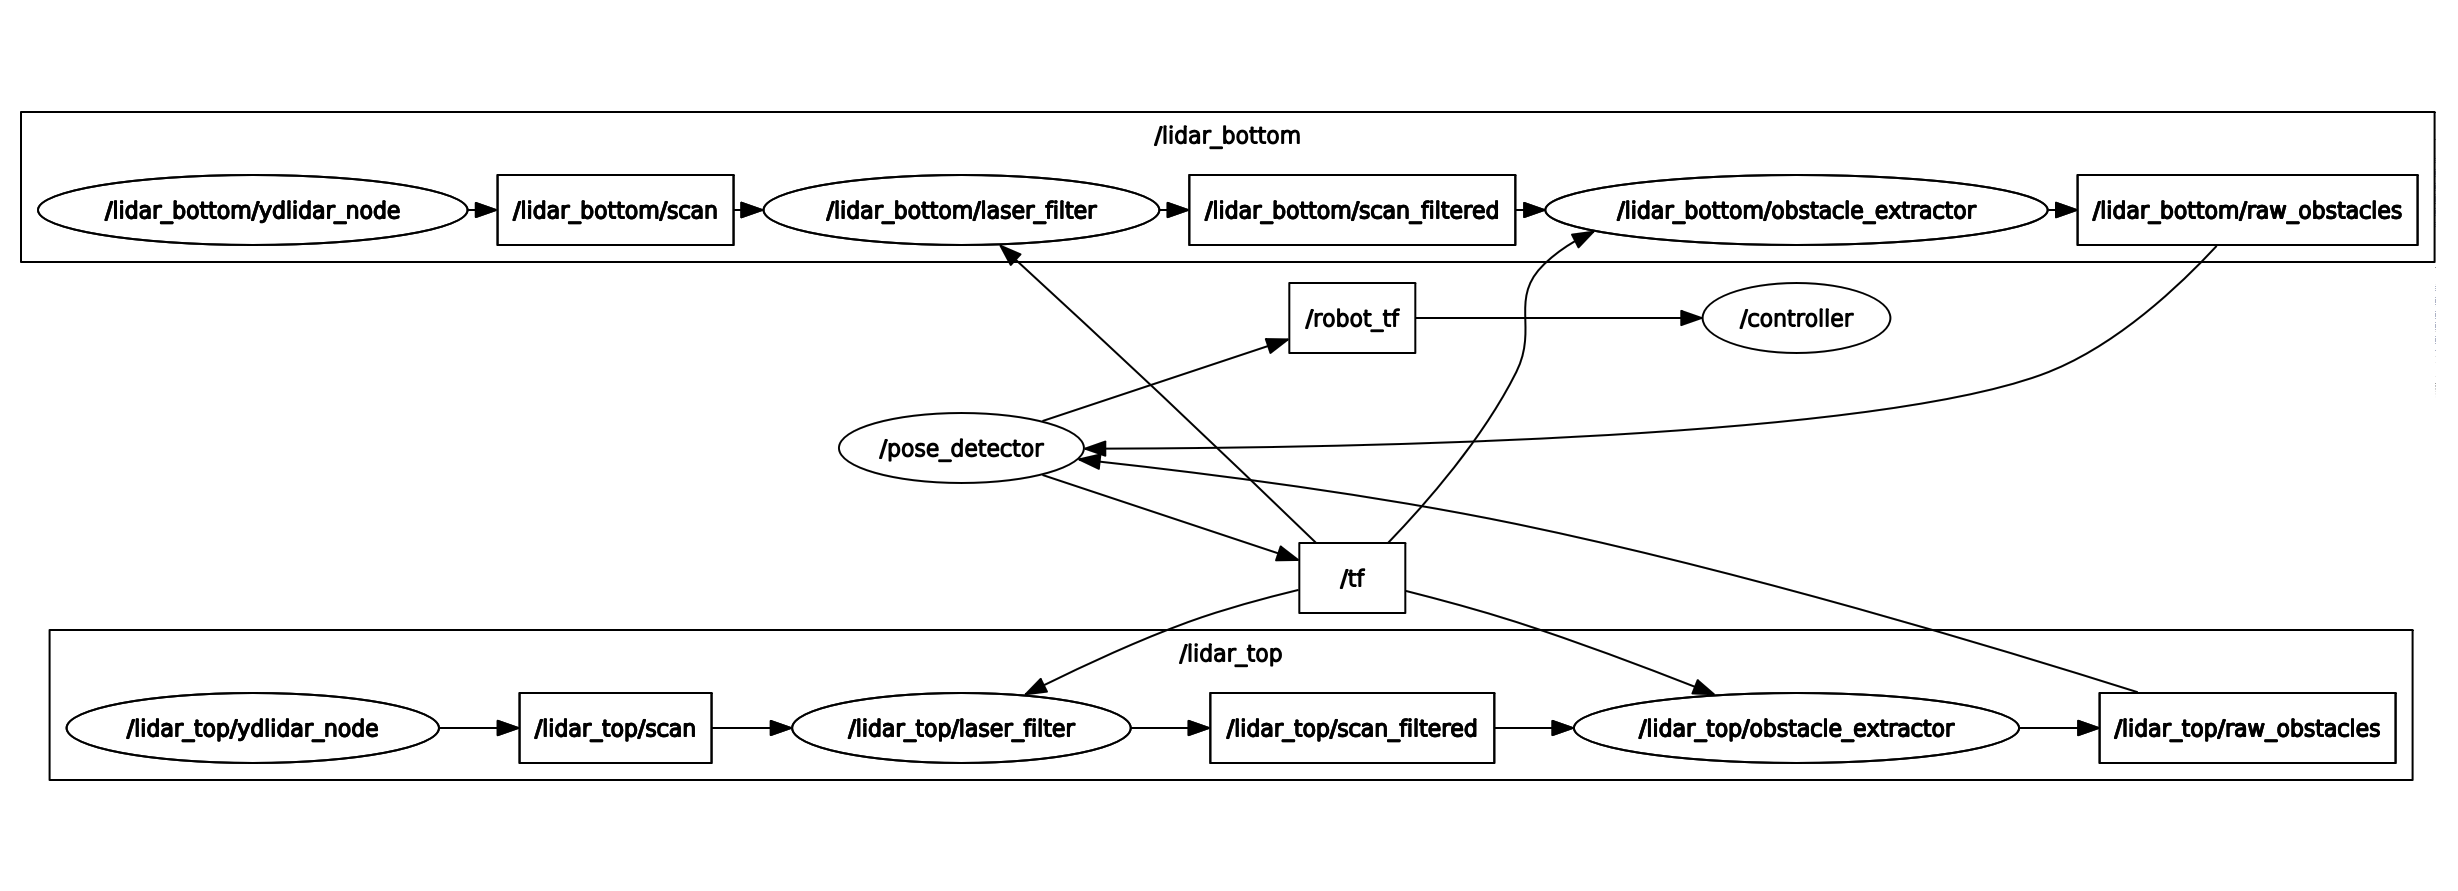
\includegraphics[width = 1.1\textwidth, frame]{./Bilder/rosgraph_nodes.png}			\caption{Relation between the nodes used in the project}
	\label{fig3}
\end{figure}


Since there are 2 sensors and the data of each sensor must be processed individually, it's important to launch separate nodes for each one. This can be done by using the attribute "ns" in the launch file. By using this attribute an instance of the node can be created in a user-defined namespace so that separate nodes are initiated. Figure \ref{fig3} shows these two namespaces, which are named "lidar\_bottom" and "lidar\_top".



As described in the previous figure, the nodes are:
\begin{enumerate}
\item \textbf{State-Publisher:} This node is responsible for publishing the jointstates and transformers of the robot.
\item \textbf{lidar\_bottom/ydlidar\_node and lidar\_top/ydlidar\_node:} These nodes publish messages of type laserscan to the topics "lidar\_bottom/scan" and "lidar\_top/scan" respectively. A LaserScan message in ROS sensor\_msgs package and it contains information about the sensor scans such as the ranges of each angle as well as the scan time and maximum and minimum range. \cite{noauthor_sensor_msgslaserscan_nodate}
\item \textbf{lidar\_bottom/scan\_filter and lidar\_top/scan\_filter} These nodes subscribe to the scan topics which are published from the ydlidar\_node and publish a filtered laserscan message to the topics "lidar\_bottom/filtered\_scan" and "lidar\_top/filtered\_scan". The scan\_filter nodes in each sensor use LaserScanBoxFilter, which exclude scan points that are outside a defined room\citep{foote_laser_filters_nodate}. The room is defined by two points in an XYZ-space. This is important to exclude the scan points of the room's walls. By doing this, only the scan points of the robot are going to be considered. Figure \ref{fig4} shows the plan view of the room, and the position of the sensors as well as the coordinates of the room. The XY coordinate of the sensors is (0,0), and the room's length as well as the room's width, is 1.6 meters. The sensor is placed 15 cm apart from the wall in both x and y directions. It's therefore concluded that  $P_{min}$ = (0.15,-0.15) and $P_{max}$ = (-1.45,1.45). 
\begin{figure}[ht]
	\centering
	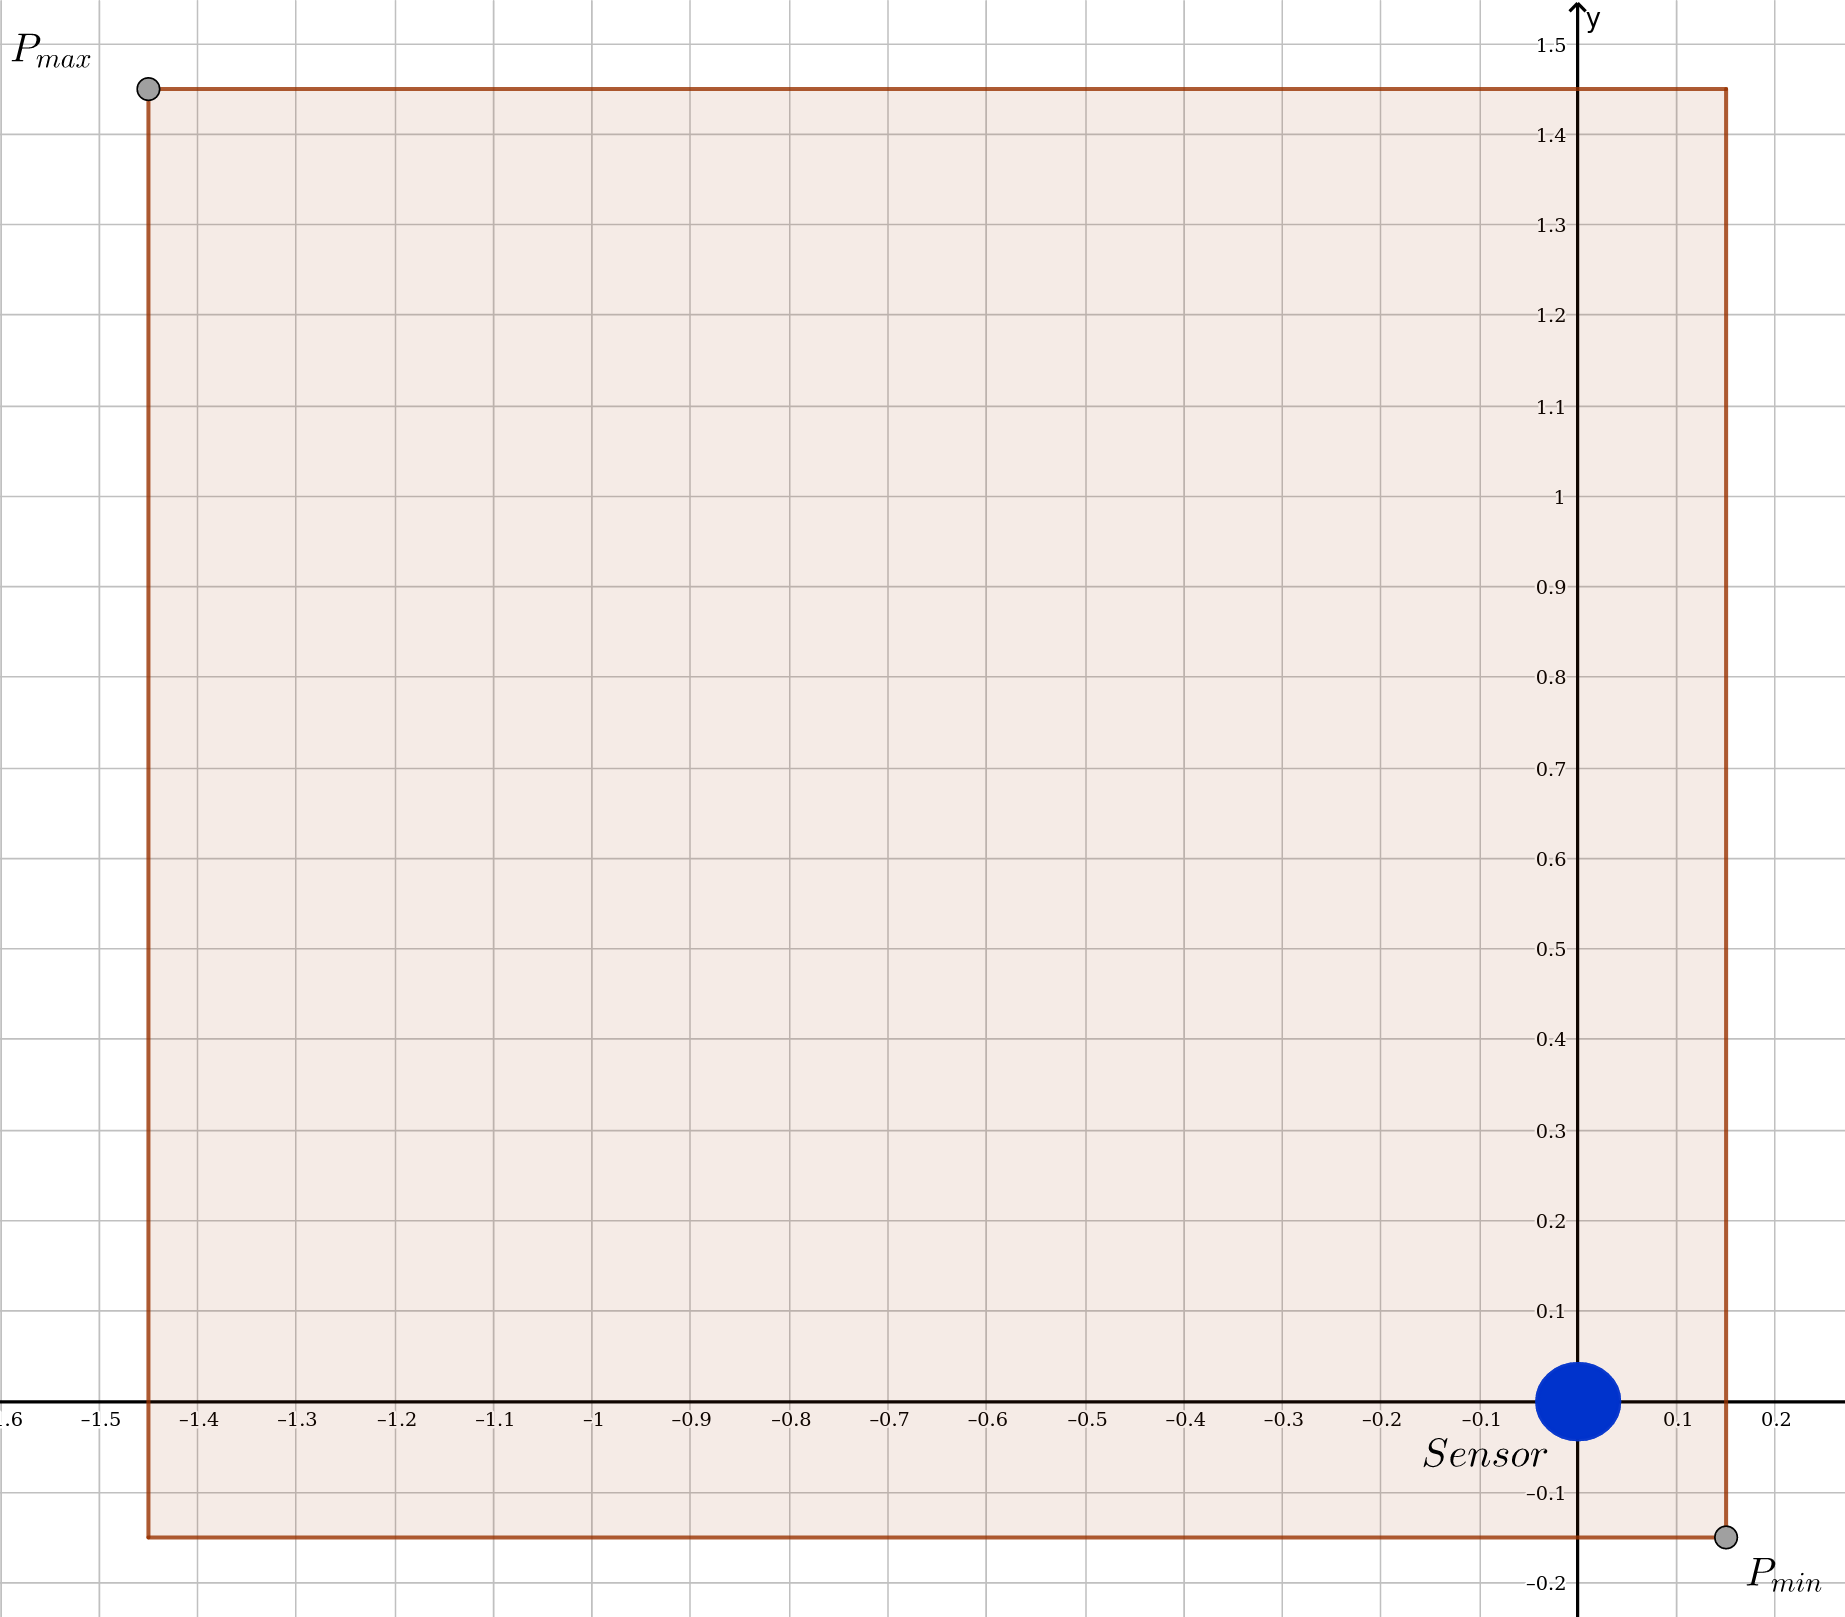
\includegraphics[width = 0.6\textwidth, frame]{./Bilder/room.png}			\caption{Plan view of the room}
	\label{fig4}
\end{figure}

\item \textbf{lidar\_top/obstacle\_extractor and lidar\_bottom/obstacle\_extractor:} subscribe to the scan\_filter topic of each sensor and  publish messages of type Obstacles to the topics "/lidar\_top/raw\_obstacles" and "/lidar\_bottom/raw\_obstacles."

\item \textbf{Pose\_Detector:} This node subscribes to the raw\_obstacle topic of each sensor and publishes the pose of the robot as a transformer message to the topic "robot\_tf". 

\item \textbf{Controller:} This node subscribes to the robot pose and publishes calculates the velocities of the left and right wheels. Then it sends velocity commands to the control unit. The implementation of obstacle extractor nodes as well as the pose\_detector node and controller node is discussed in further sections.
\end{enumerate}

\section{Robot architecture and visualization}

The design and visualization of the required system are two other building blocks that are essential for the successful completion of the project. This system consists of three main components, namely the robot, the sensors, and the room. In the first subsection, the specifications and requirements of each component in the system are explained in detail. Based on these requirements and specifications, the design of each component is going to be explained. \\
Visualizing various components of the system, including the robot, using visualization tools provided by the ROS are important for tracking results and monitoring the robot's motion.  In the second subsection, the visualization of the robot (system) in rviz is explained as well as the implementation of the robot's URDF.  

\subsection{Robot (System/Environment) design}

\textbf{System requirements:\\}
The first requirement of the system concerns the robot and sensor design. These two components must have a design that facilitates the localization process of the robot for the triangulation sensors to detect the position as well as the orientation of the robot. \\
The second requirement concerns the room design as it must be rectangular or square-shaped. Besides, the floor of the room must be a whiteboard and the sensors must be placed at a corner of the room. Lastly, the area of the room must be large enough for the robot to navigate within, yet not too large to ensure precise detection of the robot pose.

\textbf{System specifications:\\}
Some of the specifications of the robot are already known since they are closely tied to the Lego Move Hub specifications, referred to in Appendix X,  because it is the main control unit of the robot. However, other specifications must be included that are based on the requirements discussed above.
\begin{enumerate}
\item Communication Protocol:
Move Hub uses a Bluetooth Low Energy (BLE) processor for the communication between the control unit and the PC. The Bluetooth communication is based on GATT protocol.
\item Steering system:
Since Move Hub has two separated motors, each controlled individually, then the steering system of the robot is differentially steered. This steering system is nonholonomic.
\item Robot design:
The design of the robot and is related to the first requirement mentioned previously. After several trials with different designs, a specific design was achieved as follows:
\begin{itemize}
\item The robot has two cylinders with the same radius. One of these cylinders is placed at the front and the other at the back of the robot. 
\item The cylinders are placed in different XZ planes. 
\item  The cylinders are wrapped with non-reflective papers, so that the laser doesn't reflect and lead to data loss. 
\end{itemize}
The following figure \ref{fig:fig5} shows the design of the robot. The design is made by Mecabricks.com which is a web service to design models using Lego bricks. 
\begin{figure}[ht]
\begin{subfigure}[c]{0.5\textwidth}
  \centering
  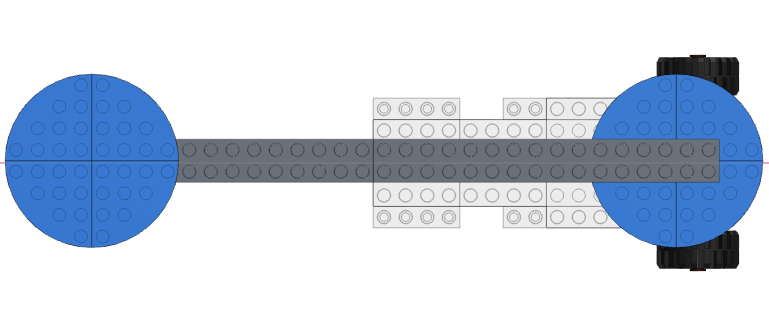
\includegraphics[width=1\linewidth]{./Bilder/Robot_Top.png}
  \caption{Plan view}
  \label{fig5:sfig1}
\end{subfigure}%
\begin{subfigure}[c]{0.5\textwidth}
  \centering
  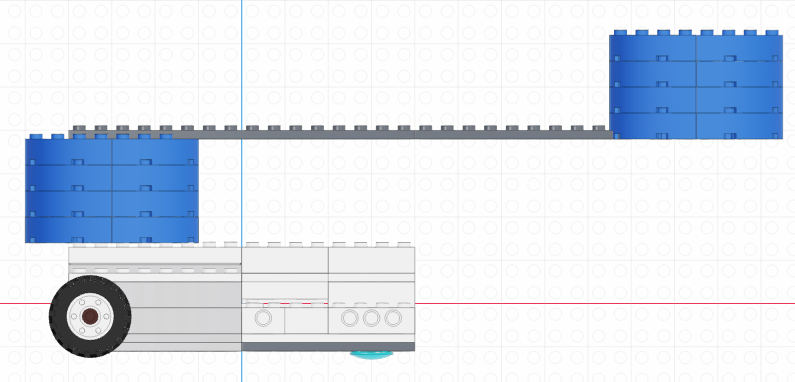
\includegraphics[width=0.8\linewidth]{./Bilder/Robot_Side.png}
  \caption{Side view}
  \label{fig5:sfig2}
\end{subfigure}
\caption{Plan and side view of the robot.}
\label{fig:fig5}
\end{figure}
\item Sensors design:
The system has 2 sensors each determine a different cylinder. The sensors are placed on each other with the same orientation, so that the x and y-axis of both sensors are identical. The sensor which is placed on top is on the same plane as the cylinder which is placed on top. The same applies to the other sensor. 
\item Room design:
The fifth specification is the design of the room and is related to the second requirement mentioned in the requirements above. To design the room, it's important to consider two aspects. The first one is  the sensor's specifications, which are discussed in section \ref{sec:lidar}. The second aspect is the ability of the obstacle detector algorithm, which is used to detect the cylinders. By considering these aspects, the maximum area of the room can be determined as follows.\\
The angle increment of the sensor is 0.72 $\frac{degree}{step}$. To detect obstacles using the obstacle detector algorithm at least 5 laser beams of the object must be valid. The first and the last beam values are actually the tangents of the cylinder. The minimum valid angle between those tangents indicates the maximum length between the sensor and the obstacle. This angle is calculated as follows: 
\begin{equation}
\theta_{min} = i*R_{min}
\end{equation}
where \hspace{15mm} $i$  =  angle increment\\ 
	  \hspace*{25mm} $R_{min}$  =  minimum number of ranges

The challenge now is to find this maximum length using this angle. This can be done by basic geometry rules. The following figure \ref{fig6} shows circle B which has a radius. The tangents of the circle are connected to the same point $A$. Theta is the angle between the tangents. 

\begin{figure}[ht]
	\centering
	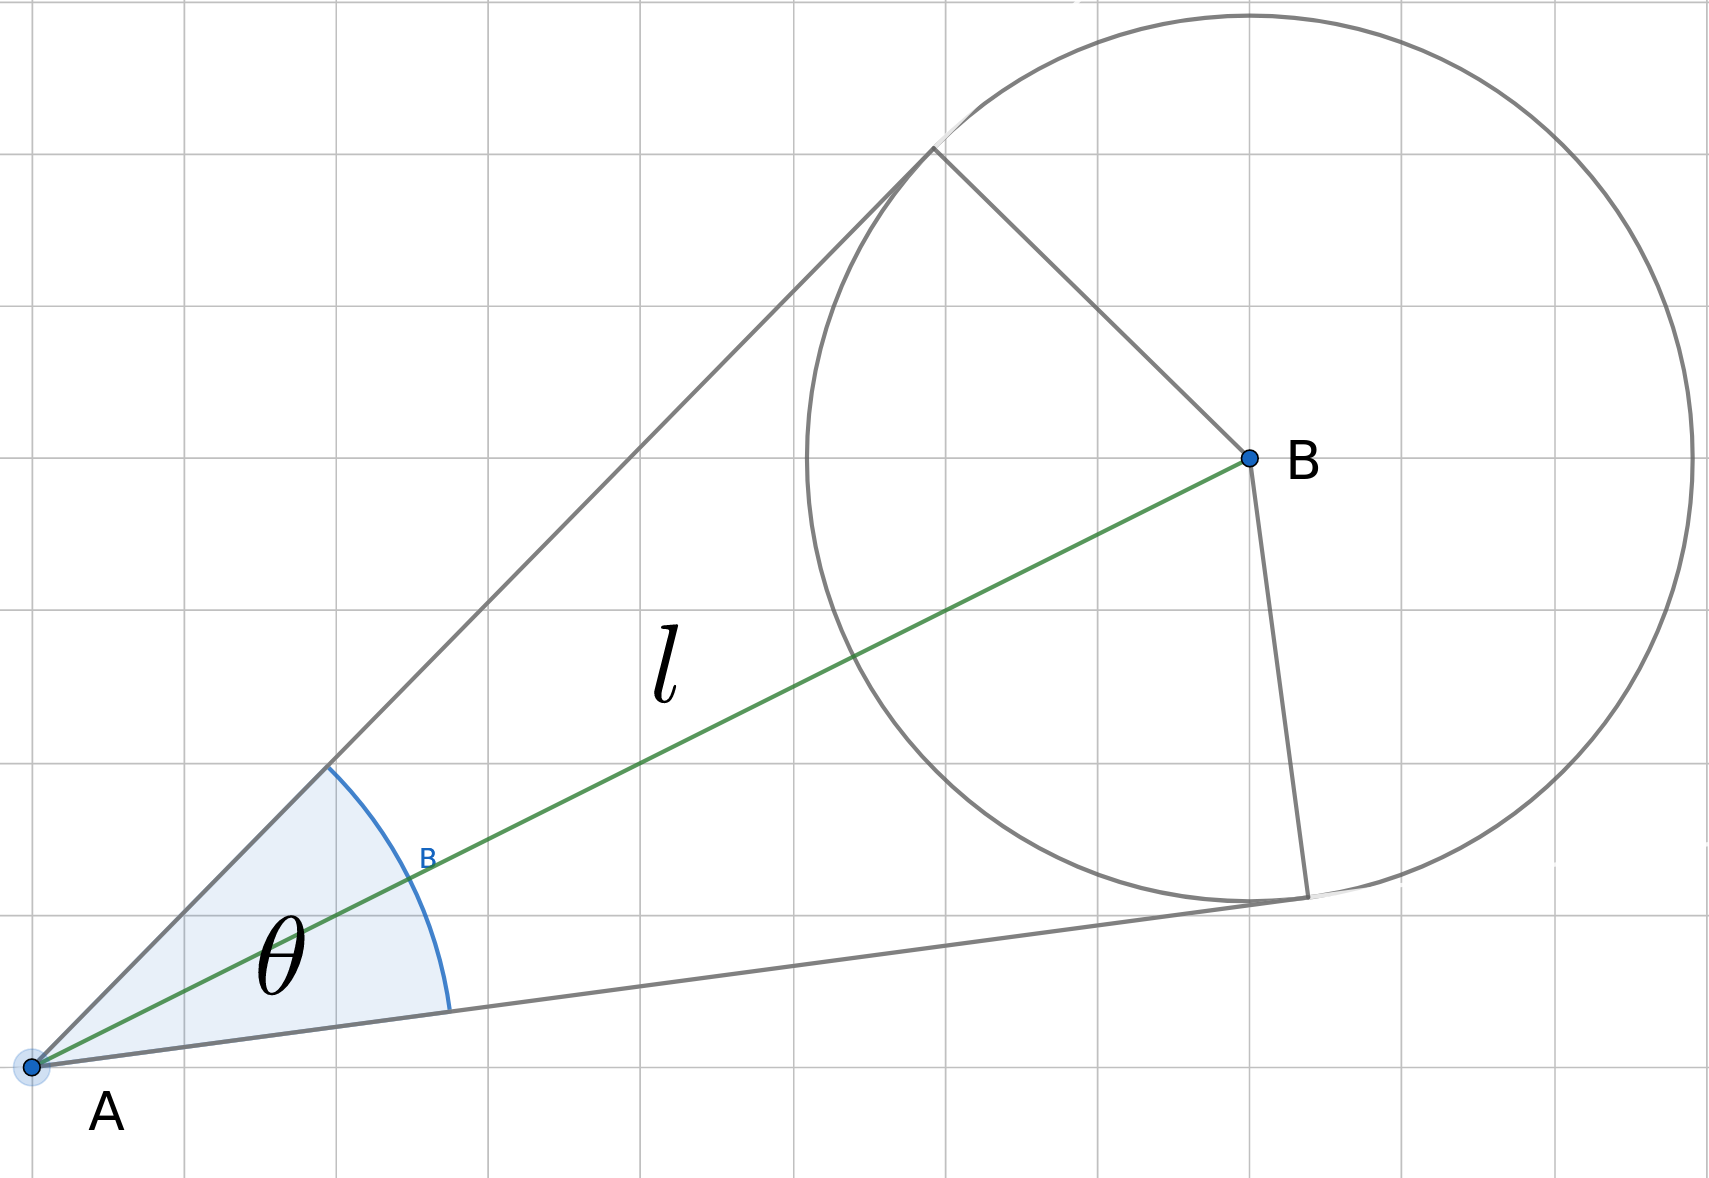
\includegraphics[width = 0.6\textwidth, frame]{./Bilder/geogebra.png}			\caption{The Relation of the length between external point and center of a circle and the angle between circle tangents to this point}
	\label{fig6}
\end{figure}


The length $l$ can be calculated as follows:
\begin{equation} \label{eq1}
l= \frac{r}{sin(\frac{\theta}{2})}
\end{equation}

by substituting theta from equation (1) in equation (2):
\begin{equation} \label{eq2}
l_{max} = \frac{r}{sin(\frac{i*R_{min}}{2})}
\end{equation}
where \hspace{15mm} $i = 0.72 \hspace{1mm}\frac{degree}{step}$\\ 
	  \hspace*{25mm} $R_{min} \geq 5$ steps
	  
From this equation, the room dimensions could be specified. By using cylinders with radius $r$ = 62 mm. Then $l_{max}$ = 2.5 m. The maximum distance in the room is the diagonal. The length of each side of the room could be calculated by using the following equation:
\begin{equation} \label{eq3}
a = \frac{l_{max}}{\sqrt{2}} = 1,768 m
\end{equation}
Yet it's important to consider the error analysis of the previously discussed method. Since the Lidar sensor has a relative error of 1.5\% for any distance between 0.5 m and 6m, and since there are 2 different sensors, then FRAGE(Error calculation)
\end{enumerate}

\subsection{Robot/Model Visualization}
Visualizing the robot and the other components of the system using visualization tools that are provided by ROS is important for watching the results and monitoring the robot motion. The visualization tool used in ROS applications is called RViz, which is a GUI used to subscribe to topics and visualize the data in these topics. RViz contains specific display types for specific message types. For example, LaserScan display type displays the data from a sensor\_msg::LaserScan message. However new display types could be added by using user-defined plugins. For example an obstacle display type is added to Rviz using a user-defined plugin. Another display type is the Robot Model, which represents the robot pose depending on its URDF. The URDF is an XML file which describes the joints and the links of the robot and the relation between them.\cite{noauthor_urdfxmljoint_nodate}




 That being said, the next step is to write the URDF file of the LegoBoost robot.  The URDF of LegoBoost robot is simple. It consists of 4 links and 3 joints. The first joint is the base joint, which connects between two links, namely the base footprint which is the parent link, and the base link which is the child link. The base footprint demonstrates the position of the robot at the ground level. The base link is the position of the center of mass of the robot. It's placed above the base footprint\cite{noauthor_rep_nodate}. These two links are connected through a fixed joint named base joint. The base joint is fixed since it doesn't have any degree of freedom. The second joint is the right wheel joint, which connects the base link to the right wheel link. The last joint is the left wheel joint, which connects between the base link and the left wheel link. The hierarchy of the URDF  and the connection between the different links and joints is shown in figure \ref{fig7}. This figure is generated by urdf\_to\_graphviz tool.

\begin{figure}[ht]
	\centering
	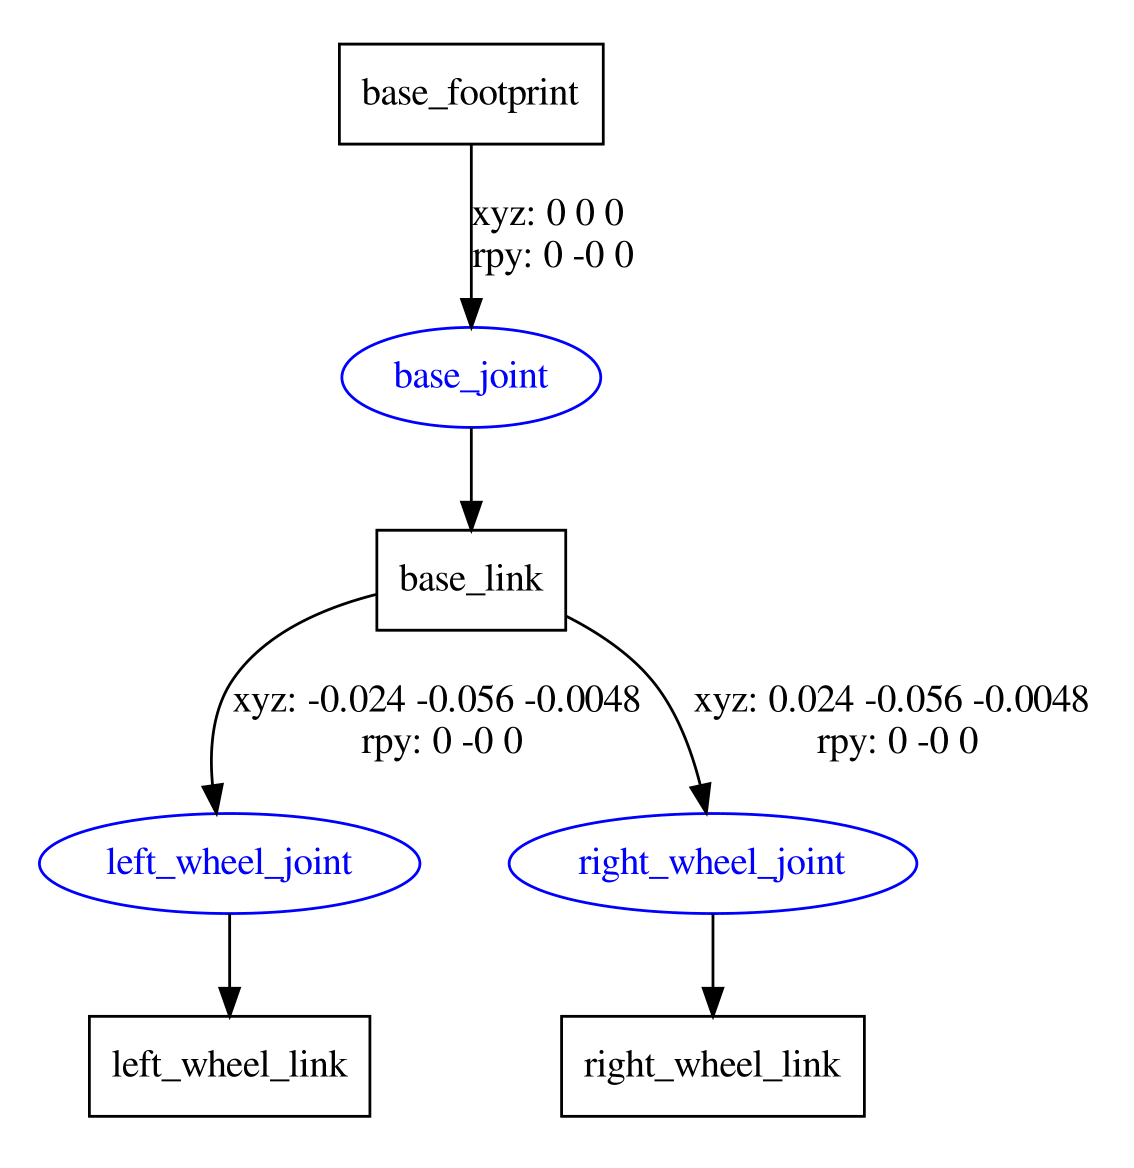
\includegraphics[width = 0.6\textwidth, frame]{./Bilder/legoboost_robot.png}			\caption{Graphical demonstration of LegoBoost URDF}
	\label{fig7}
\end{figure}


Each link in the URDF file can contain visual properties. The visual properties could be used for a better visualization of the robot. The geometry of both right and left wheel links are implemented in the URDF as cylinders with the same radius of the robot's wheels. The base link geometry is implemented as a box with the same dimensions of the robot.\\
After implementing the URDF file, the next step is to set up the Rviz tool and add all the required display types, which are:
\begin{itemize}
\item Robot model: This displays the URDF of the robot.
\item LaserScan: This displays the scan data of the sensors. A LaserScan display type is added for each sensor.
\item Obstacles: This displays the cylinders on the robot. An obstacle is added to each cylinder. Each cylinder is colored differently, namely red for the top cylinder and blue for the bottom cylinder. 
\item TF: This displays the TF transform hierarchy of the model. 
\end{itemize} 
The final visualization of the whole model in RViz is shown in figure \ref{fig8}. The frames of the sensors as well as the robot are demonstrated. The red and white points demonstrate the laserscans of the sensors and the red cylinder shows the front cylinder of the robot. The cylinder at the back is not shown in this figure for simplicity and clearer vision.
\begin{figure}[ht]
	\centering
	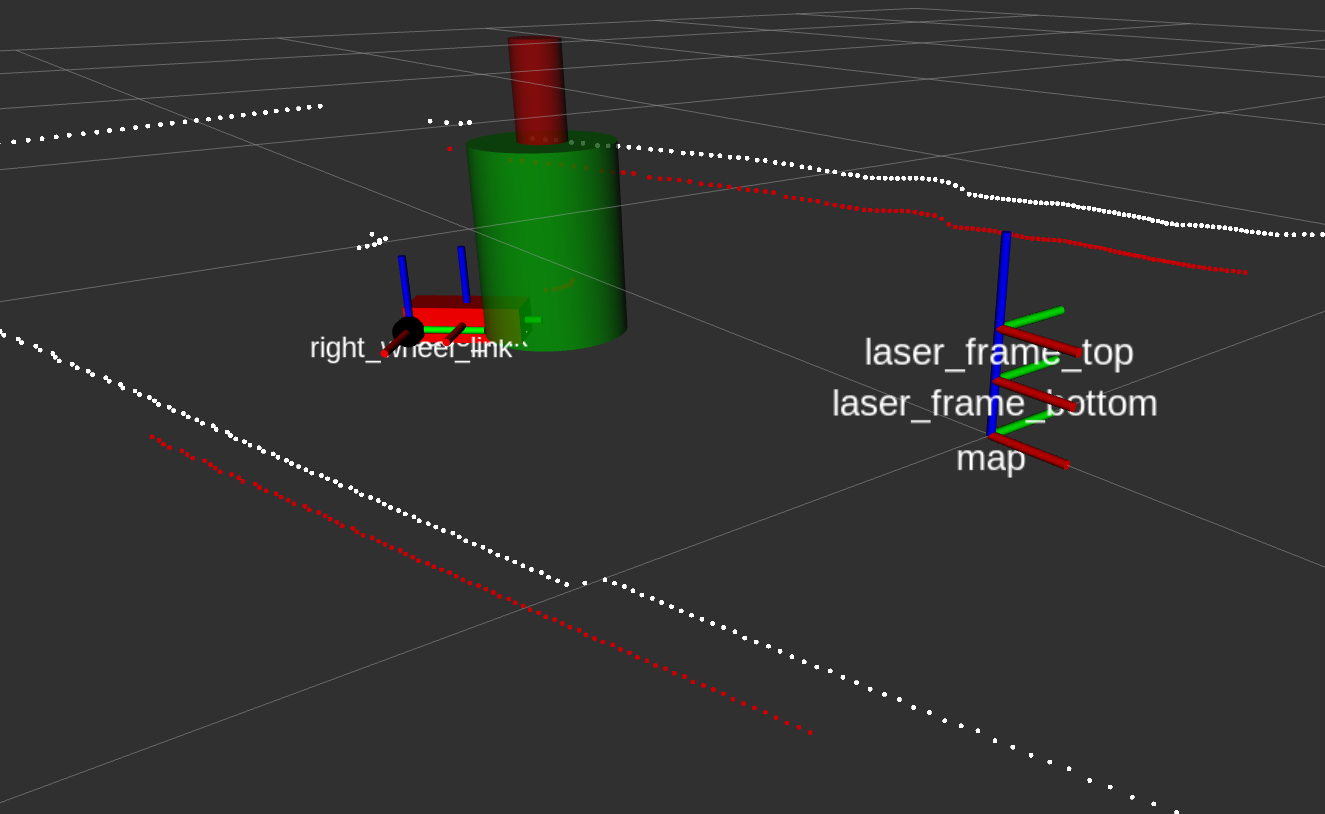
\includegraphics[width = 0.9\textwidth, frame]{./Bilder/rviz_screenshot.png}
	\caption{The model visualization in RViz}
	\label{fig8}
\end{figure}

\section{Robot localization}
Robot localization is another essential building block in the project and the core of the thesis.   Under robot localization two things must be considered. First, is localizing the position of the robot, and second, localizing the orientation of the robot. Both the orientation and the position represent the pose of the robot. Localization in mobile robots context is usually performed by using SLAM algorithms, where a lidar sensor or a camera is integrated in the robot to scan the surrounding environment and the SLAM algorithms are used to build a map of this environment and localize the pose of the robot depending on this map and other inputs like the odometry of the robot \cite{ros_book}. In contrast to the SLAM algorithms, the method used in this thesis is however different, since the sensors are not integrated in the robot but fixed in a specific place in the room. From the perspective of the sensor, the surrounding environment is still, and only the robot is moving. In this section, the used methods, which have been used for the robot localization are going to be discussed. Firstly, localization using the obstacle detector approach is discussed. Then the localization using image processing is discussed. At last, the localization using laser scan matcher approach is discussed.

\subsection{Circular object detection approach}   %8 pages
%1)introduction and explain how the algorithm work   1page
%2)how did I implement the approach to detect the robot pose 6pages
%	2.1 Idea explanation (Geometry)
%	2.2 Code explanation
%3)how accurate is the detection 1 page
%4) conclusion 1 page


Obstacles detection algorithms are essential in robot navigation. Such algorithms are used for example during navigation to avoid obstacles. The obstacle detection algorithm developed in \cite{obstacle_detector} is used for detecting circle-shaped obstacles by using circles geometric properties and the polynomial regression of laser scan data. The main reason for choosing this algorithm is its fascinating efficiency and speed. According to the applied tests mentioned in \cite{circle} the accuracy rate of the circles' detection is 92.53\% and the average executing time is 16 $ms$ per frame which is around $50 Hz$. This is more than twice the publishing rate of the sensor, which is $20 Hz$.  The main idea of using this algorithm is to detect the cylinders, that are placed on the robot. By detecting the exact position of these cylinders, the pose of the robot could be calculated. 



\subsection{Image Processing approach} %4 pages
%1)introduction and explain how the algorithm work
%2)how did I implement the approach to detect the robot pose
%	2.1 Idea explanation (Geometry)
%	2.2 Code explanation
%3) Difficulties, and why didn't I continue working on this approach


\subsection{Laser scan matcher approach} %4 pages
%1)introduction and explain how the algorithm work
%2)how to implement the laser scan matcher. which data are used as inputs and %what is the output of the algorithm (Computational graph)
%3) Difficulties, and why didn't I continue working on this approach


